\subsection{Element-Mesh relations -- ELE-MSH}
\label{sec:ele_msh}

From Fig. \ref{fig:ele_objects} it can be seen, that element-mesh
relations have multiple functions in the element concept, e.g.
\begin{itemize}
 \item ELE-GEO relation: mesh topology, neighbor relationships of
 geometric elements, element connectivity, incorporation of of boundary
 conditions,
 \item ELE-FEM relation: coordinate transformation between local
 element and global coordinates,
 \item ELE-PCS relation: local element nodes and node index in the
 global equation system, material domains.
\end{itemize}

\subsubsection{ELE-GEO relation}

Apart from the individual/intrinsic element properties, the
\texttt{ELEM} object contains information about mesh topology,
i.e. how this element is emplaced in the element mesh. For
instance, the (\texttt{sub\_domain}) index indicates the part of
the domain to which this element belongs. This number is used e.g.
to distinguish elements in different areas of the domain with
different material properties. Neighbor relationships of geometric
elements are important topological properties of an element mesh.
Neighbors of an element are all those elements adjacent to the
faces of the element. Since the definition of \texttt{ELEM} object
provides necessary functionality of different geometric element
types, we use pointers to \texttt{ELEM} object itself to recode
neighbors as

\texttt{Vector$<${}CElem$\ast>${}\ neighbors;}

\begin{figure}[H]
 \centering
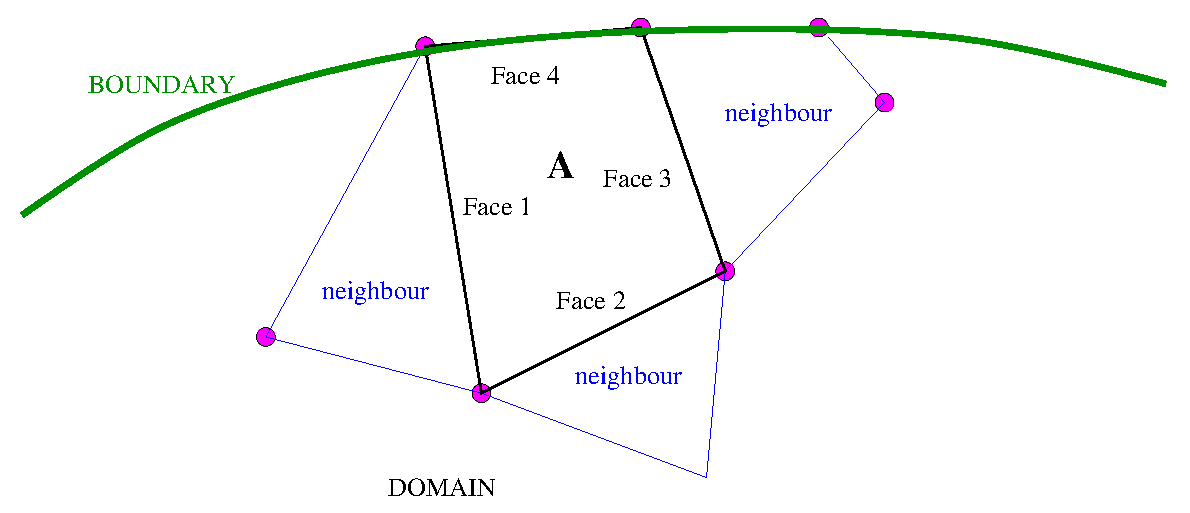
\includegraphics[scale=0.6]{figures/neighbor.eps}
\caption{Definition of element neighbors} \label{fig:gnei}
\end{figure}

As an example Fig. \ref{fig:gnei} illustrates the arrangement of
neighbor relationships in 2D space, in which quadrilateral
element A has three neighbor elements adjacent to its faces (i.e.
edges in 2D) 1, 2 and 3. Neighbors 1 and 2 are triangle elements,
while neighbor 3 is a quadrilateral element. Face 4 is on the
domain boundary, which is not shared by any other element. Vector
member, \texttt{neighbors}, is initialized with size of 4 and
assigned during mesh construction. The first three entries are
assigned with pointers to neighbors 1, 2 and 3. The last entry of
the vector is filled with a pointer to a surface (Face 4), which
is an instance of \texttt{ELEM} object configured for a line
element. The boundary type \texttt{position} of this instance is
set as 'B'. The coding of the element neighboring process is given
below:

\small
\begin{center}
\begin{verbatim}
neighbors[0] = (CElem*) Neighbour1;
neighbors[1] = (CElem*) Neighbour2;
neighbors[2] = (CElem*) Neighbour3;
neighbors[3] = (CElem*) Face4;
Face4->position = 'B'; // on domain boundary
Face4->owner = this; // this element
\end{verbatim}
\end{center}
\normalsize

The above neighbor vector is a member of element,
i.e., ELEM, object.

\subsubsection{ELE-FEM relation}

The ELE-FEM association concerns coordinate transformation between
local element and global coordinates. Depending on the geometric
and numerical type of a finite element, related shape functions
and their derivatives are available (section \ref{sec:ele_fem}).
%%This is particularly important for hybrid meshes (Fig.
%%\ref{ffig:gnei}). 
Jacobian calculations are another typical ELE-FEM methods.

\subsubsection{ELE-PCS relation}

Subdomain properties of element are used to describe heterogeneity, 
i.e. local variation of material properties for different problems. 
Element neighbor relationships are essential data for constructing 
the mesh and determine the propagation orientation of 
discontinuities in failure analysis (section \ref{sec:apl_m}). 
Moreover, the proposed element concept allows the assignment of 
different processes (PCS objects) and meshes (MSH objects). 
%%This is an important feature for upscaling procedures \cite{Kol:2005b}.
